\documentclass{article}

\usepackage[utf8]{inputenc}  % For encoding support
\usepackage{amsmath}         % For mathematical formatting
\usepackage{graphicx}        % For including images
\usepackage{xcolor}
\usepackage[a4paper, left=0.5in, right=0.5in, top=0.5in, bottom=0.5in]{geometry}  % Adjust margins here

\title{Compiler Design Notes}
\author{Ayush Raina}
\date{\today}

\begin{document} 

\maketitle

\section*{Control Flow Analysis}
\subsection*{Why Control Flow Analysis?}
Helps to understand structure of Control Flow Graph (CFG), To detect loops in the CFG, Dominator Information,Dominator Frontier Information required for Single Static Assignment (SSA) form. Interval Information used in Data Flow Analysis, Control Dependence Information used in Parallelization.

\subsection*{Dominators}
\begin{enumerate}
    \item We write $(d \text{ dom } n)$ if every path from initial node $n_0$ to node $n$ passes through node $d$. A node dominates itself.
    \item Node $x$ strictly dominates node $y$ if $x$ dominates $y$ and $x \neq y$.
    \item $x$ is immediate dominator of $y$ if $x$ is closest strict dominator of $y$.
\end{enumerate}

\subsection*{Algorithm to find Dominators}
Let us denote the set of Dominators of node $n$ as $D(n) = OUT(n)$. These sets are very helpful to construct the dominator tree quickly. 
\begin{itemize}
    \item Start with $n_0$ such that $D(n_0) = \{n_0\}$.
    \item for each $n \in N - \{n_0\}$ do the following:
    \begin{itemize}
        \item First set $D(n) = N$.
        \item Take intersection of all the outsets of the predecessors of $n$ denoted by $IN(n) = \bigcap_{p \in pred(n)} OUT(p)$.
        \item $D(n) = IN(n) \cup \{n\}$.
    \end{itemize}

    \item Repeat until $D(n)$ stabilizes for all $n$.
\end{itemize}

\subsection*{Back Edges and Natural Loops}

\textbf{Back Edges: } Edges whose head dominates the tail are called back edges. To find the back edges, one easy way to look if opposing edges according to dominator tree is present in the graph. \\
\textbf{Natural Loops: } Given a back edge $(n,d)$, the natural loop of the edge is $d \cup $ all the nodes that reach $n$ without going through $d$. In this case $d$ is the header of the loop and dominates all the nodes in the loop.

\subsection*{Algorithm for finding the natural loop of a back edge} 
Let the back edge be $(n,d)$. Then initialize a empty stack. Push $n$ into the stack. Initialize a vector with $d$ in it. Then until the stack is empty, pop the top element and push its predecessors into the stack. If the predecessor is not in the vector, add it to the vector. Continue until the stack is empty. The vector now contains the natural loop.

\subsection*{Depth First Numbering of Nodes in a CFG}
We start a $DFS(n)$ from initial node $n_0$ where $n$ is total number of nodes. We mark a node to $n$ when it is last visit to that node. Last visit means that all the children of that node are visited and now this node will not be visited again. Then we decrement $n$ and continue the process. This way we can number the nodes in a CFG.

\begin{figure}[h]
    \centering
    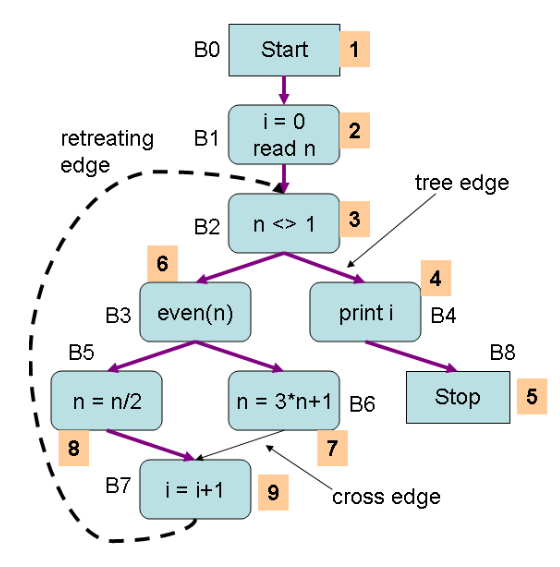
\includegraphics[width=0.5\textwidth]{Images/dfs1.png}
    \caption{DFS Numbering of Nodes}
    \label{fig:cfg}
\end{figure}

\newpage

\subsection*{Reducibility}
A flow graph $\mathcal{G}$ is reducible iff every back it can be partitioned into 2 disjoint sets of forward and back edges such that:

\begin{itemize}
    \item Forward edges form a DAG in which every node is reachable from the initial node.
    \item All the retreating edges are back edges.
    \item In an irreducible flow graph, some retreating edges will not be back edges, hence graph of forward edges will contain a cycle.
\end{itemize}

\begin{figure}[h]
    \centering
    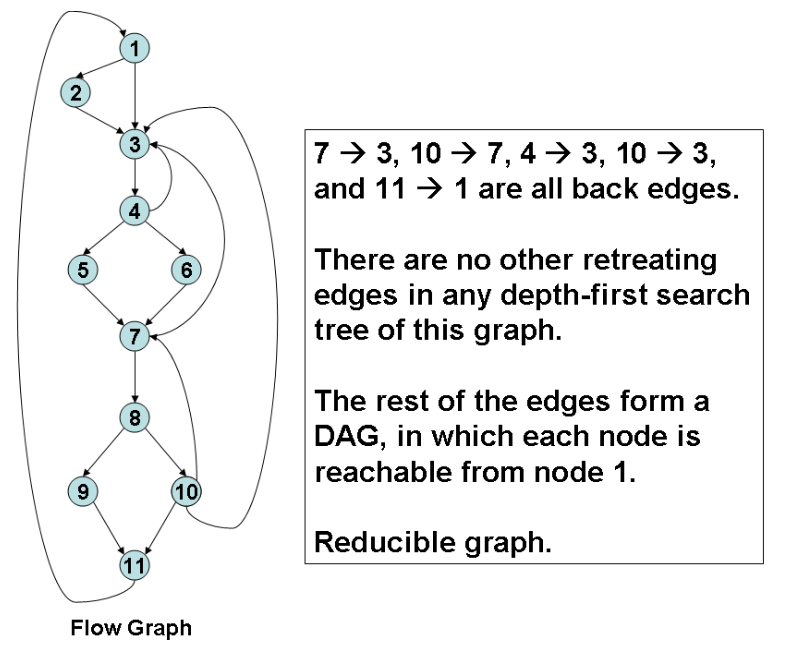
\includegraphics[width=0.4\textwidth]{Images/reducible.png}
    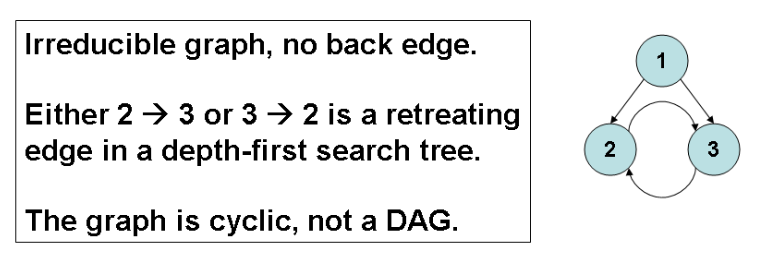
\includegraphics[width=0.4\textwidth]{Images/irreducible.png}
    \caption{Reducible and Irreducible CFG}
    \label{fig:cfg}
\end{figure}

\subsection*{Inner Loops}
Unless two loops have same header $n \longrightarrow d$ (here d is header), they are either disjoint or one is nested inside the other. If natural loop set of one header is subset of the other then there is nesting. Similarly two loops are disjoint if their natural loop sets are disjoint and two loops are identical if their natural loop sets are identical.

If two loops share a header, neither of these may hold and in such a case loops are combined and transformed.

\begin{figure}[h]
    \centering
    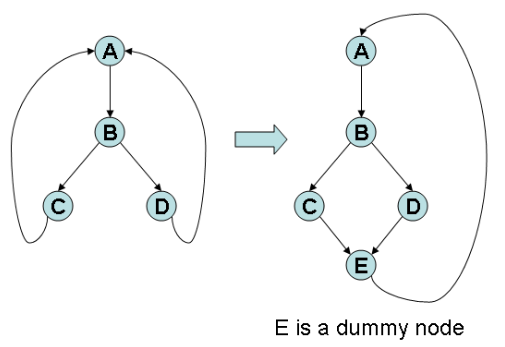
\includegraphics[width=0.4\textwidth]{Images/transform.png}
    \caption{Transformation in case of shared header}
    \label{fig:cfg}
\end{figure}

\newpage

\subsection*{Pre Header}
\begin{figure}[h]
    \centering
    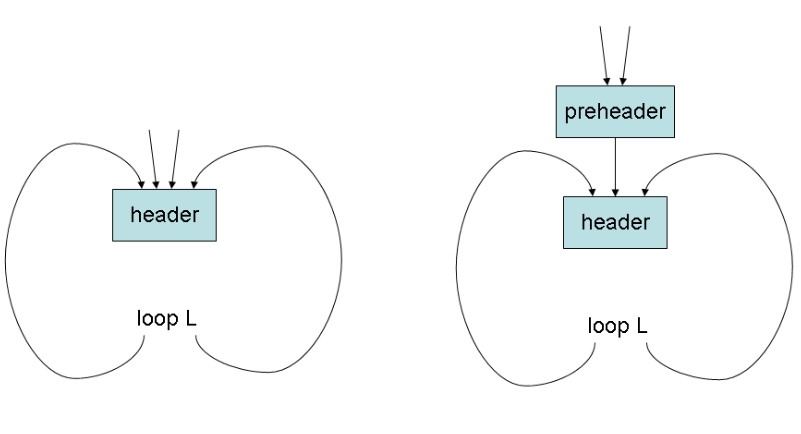
\includegraphics[width=0.4\textwidth]{Images/preheader.png}
    \caption{Pre Header}
    \label{fig:cfg}
\end{figure}

\subsection*{Depth of a CFG and Convergence of DFA Problem}
To be continued.

\newpage

\subsection*{Intervals}

Intervals have a header node which dominates all the other nodes in that interval.
Given a flow graph $\mathcal{G}$ with initial node $n_0$.The interval with header $n$ denoted by $I(n)$ is the set defined as: \\ \\
1. $n \in I(n)$. \\
2. If $\exists \; m$ such that $Pred(m) \subset I(n)$ then $m \in I(n)$. \\
3. Nothing else is in $I(n)$. \\ \\
Constructing $I(n)$: \\
1. Start with $I(n) = \{n\}$. \\
2. While there exists a node $m$ such that $Pred(m) \subset I(n)$, do $I(n) = I(n) \cup \{m\}$.

\subsection*{Paritioning a flow graph into disjoint intervals}
1. Mark all the nodes as unvisited. \\
2. Construct $I(n_0)$ and mark all the nodes in $I(n_0)$ as visited. \\
3. while there is an unvisited node $m$ with atleast one predecessor $p$ which is selected, construct $I(m)$ and mark all the nodes in $I(m)$ as visited and repeat the process. 

\begin{figure}[h]
    \centering
    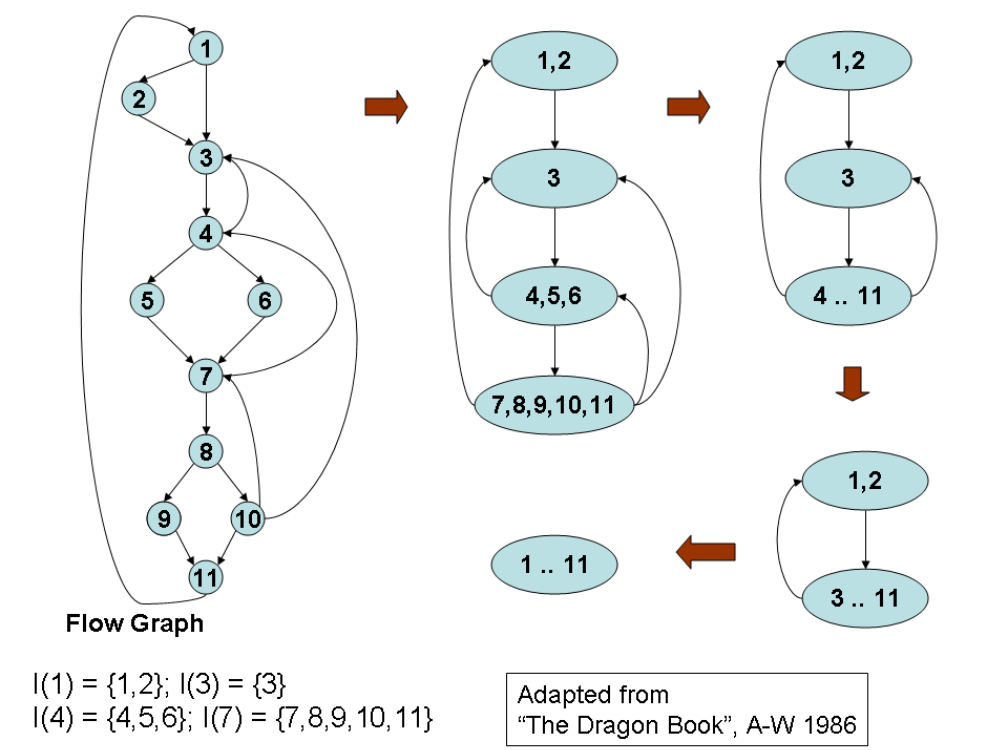
\includegraphics[width=0.7\textwidth]{Images/reducible2.png}
    \caption{Intervals}
    \label{fig:Reducibility}
\end{figure}

In 1st step we got disjoint intervals. Now in the above figure we repeat same procedure further on the interval graph until we reach single node.

\subsection*{Interval Graphs}
1. Interval graph is denoted by $I(\mathcal{G})$. Intervals correspond to nodes and interval containing $n_0$ is the initial node of $I(\mathcal{G})$. \\
2. If there is an edge from a node in $I(m)$ to the header of interval $I(n)$ then there is an edge from $I(m)$ to $I(n)$ in $I(\mathcal{G})$. \\
3. We make intervals in interval graph until we reach a limit flow graph which cannot be reduced further. \\
4. \textcolor{red}{A flow graph is reducible iff its limit flow graph is a single node.}

\subsection*{Node Splitting (Extra)}
If we reach limit flow graph which is not a single node, we can still proceed further if we split one or more nodes. \\ 
1. If a node has $k$ predecessors then we may replace $n$ by $k$ nodes $n_1, n_2, \ldots, n_k$ such that $i^{th}$ predecessor of $n$ becomes predecessor of $n_i$ and all the successors of $n$ become successors of $n_i \forall i \in [1,k]$. \\
2. After splitting the nodes, we continue reduction process and do node splitting wherever required to reach a single node limit flow graph, however success is not guaranteed. \\

\begin{figure}
    \centering
    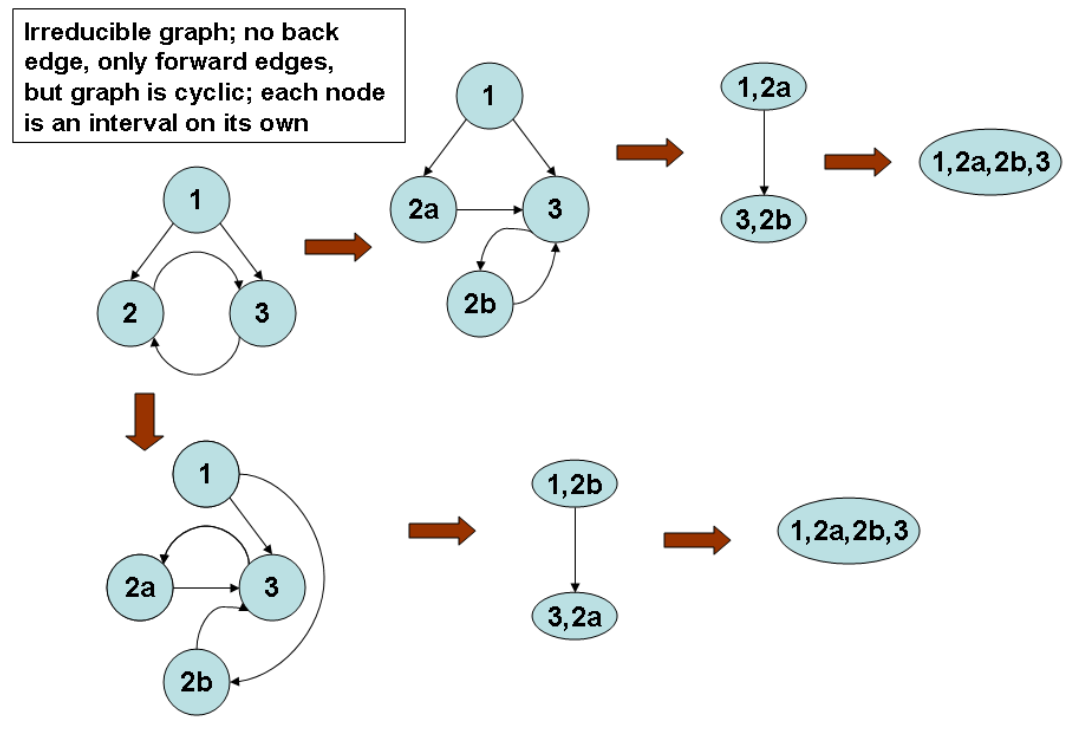
\includegraphics[width=0.7\textwidth]{Images/nodeSplit.png}
    \caption{Node Splitting}
    \label{fig:NodeSplitting}
\end{figure}

\subsection*{T1-T2 Transformations and Graph Reduction}
\textbf{T1 Transformation: }If n is a node with a loop i.e $(n \rightarrow n)$ edge exists then delete that edge. \\
\textbf{T2 Transformation: }If there is a node $n$, not the initial node with a unique predecessor $m$ then combine $n$ into $m$. \\

By Applying T1,T2 transformations in any order we may reach limit flow graph and node splitting may be required wherever necessary in order to reach a single node limit flow graph.

\begin{figure}[h]
    \centering
    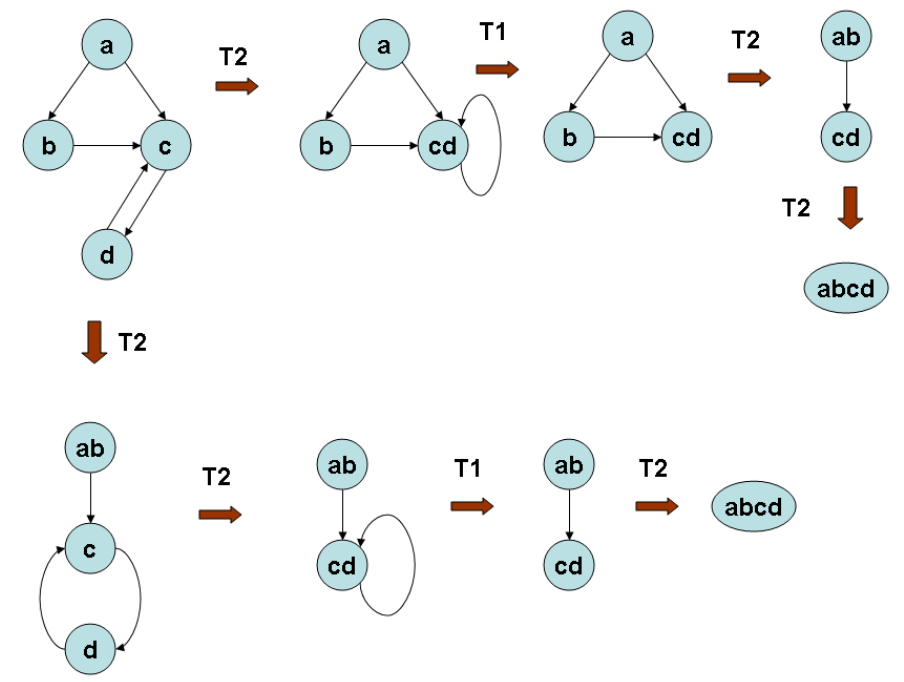
\includegraphics[width=0.7\textwidth]{Images/t1t2.png}
    \caption{T1-T2 Transformations}
    \label{fig:T1T2}
\end{figure}

One more example of a bigger CFG can be found in slides available on course webpage.

\subsection*{Regions}
A set of nodes $N$ that includes a header and it dominates all other nodes in $N$ is called region and all these edges between nodes in $N$ are in the region except (possibly) the edges that enter the header. \\
All intervals are regions but all regions are not intervals. A region may have multiple exits but an interval has only one exit. As we reduce a flow graph G using $T1-T2$ transformations, at each step the node obtained is a region.

\begin{figure}[h]
    \centering
    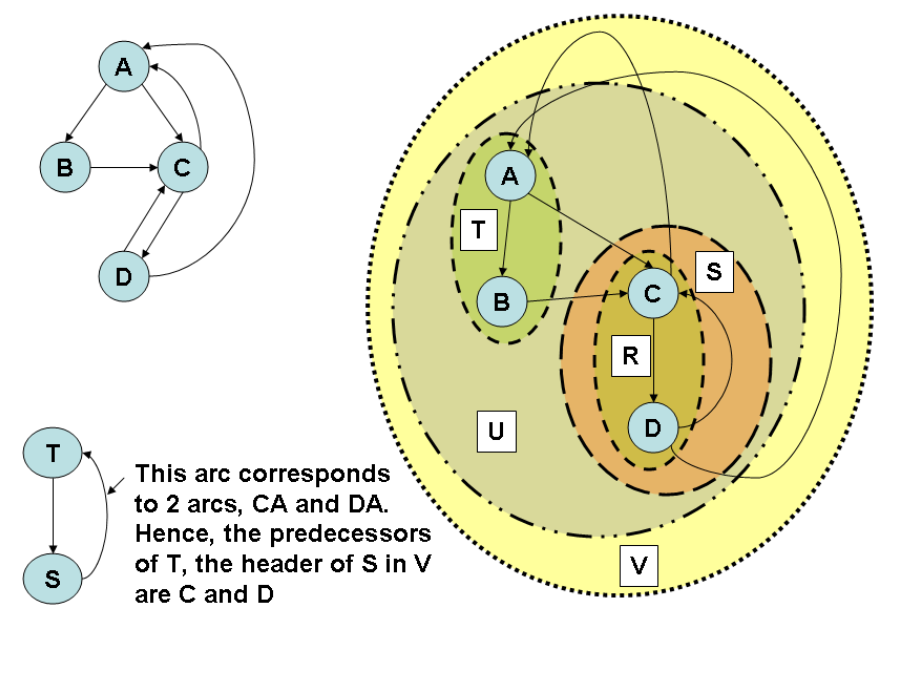
\includegraphics[width=0.7\textwidth]{Images/region.png}
    \caption{R,S,T,U,V are different regions marked}
    \label{fig:Regions}
\end{figure}

\subsection*{End of Control Flow Analysis}

\newpage

\section*{Data Flow Analysis}
These are the techniques that derive information about flow of data along execution paths. \\
An execution path from path $p_1$ to $p_n$ is sequence of points such that for each $i \in [1,n-1]$ either $p_i$ is preceeding some statement $s$ and $p_{i+1}$ is immediately following the same statement $s$ or $p_i$ is end of some block and $p_{i+1}$ is start of successor block. \\
In general there can be infinite number of paths from a program and there is no bound on length of a path. \\

\subsection*{Uses of DFA}
Common uses are program debugging and program optimizations. \\
\textbf{Program debugging: } may include what are the definitions of variables reaching a particular point ? These are reaching definitions. \\
\textbf{Program Optimization: } It includes optimizations like common subexpression elimination. \\

\subsection*{Data Flow Analysis Schema}
Let us first see some definitions: \\
1. \textbf{Data flow value: } for a program point represents an abstraction of all possible program states that can be observed from that particular point in the program. The set of all possible data flow values is called Domain of the application under consideration. \\
2. \textbf{IN(s) and OUT(s)}: represents the data flow values at beginning and end of each statement $s$. \\
3. \textbf{Data Flow Problem:} is to find a solution to set of constraints on $IN(s)$ and $OUT(s)$ for all statements $s$. These constraints are of two types: constraints based on semantics of statements such as transfer functions and constraints based on control flow such as if-else conditions. \\
4. \textbf{Safe Estimates: } A decision or estimate is safe if it never leads to a change in what is being computed in the program (after the change).  \\

A DFA schema consists of: \\    
1. Control Flow Graph (CFG) \\
2. Direction of Data Flow (Forward or Backward) \\
3. Set of Data Flow Values (Domain) \\
4. Confluence Operator \\
5. Transfer Functions for each block \\

\section*{Reaching Definitions} 
Purpose of reaching definitions is to perform optimizations by computing loop invariant. A definition $d$ reaches a point $p$ if there is a path from the point immediately following $d$ to $p$ such that $d$ is not killed on that path. We say a definition of a variable is killed if between 2 points along the path, there is re-assignment to the variable. \\

The data flow equations(constraints) are as follows: Initialize $IN(B) = \phi$ for all blocks $B$. If some definitions reach $B_1$ (entry block) then $IN(B_1)$ is initialized with those definitions. Then we have: \\
1. $IN(B) = \bigcup_{p \in pred(B)} OUT(p)$ \\
2. $OUT(B) = GEN(B) \cup (IN(B) - KILL(B))$ \\

This is a forward $DFA$ problem since $OUT(B)$ is computed in terms of $IN(B)$ and Confluence operator is $\cup$. $GEN(B)$ is the set of definitions which are visible immediately after the block $B$ and $KILL(B)$ is the union of  definitions in all basic blocks which are killed by individual definitions in $B$. Here is an example of reaching definitions:

\begin{figure}[h]
    \centering
    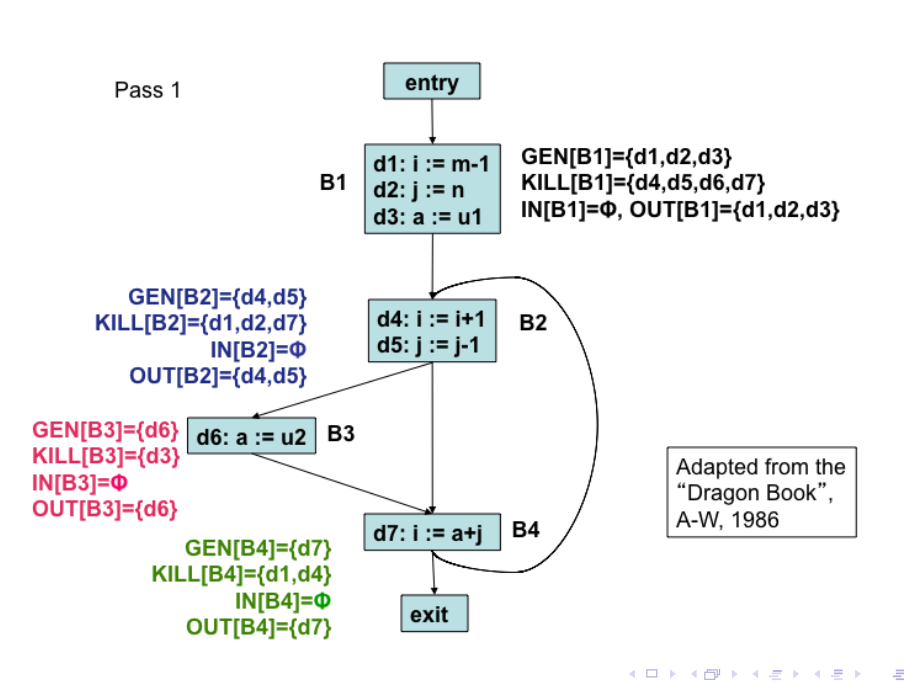
\includegraphics[width=0.4\textwidth]{Images/reaching1.png}
    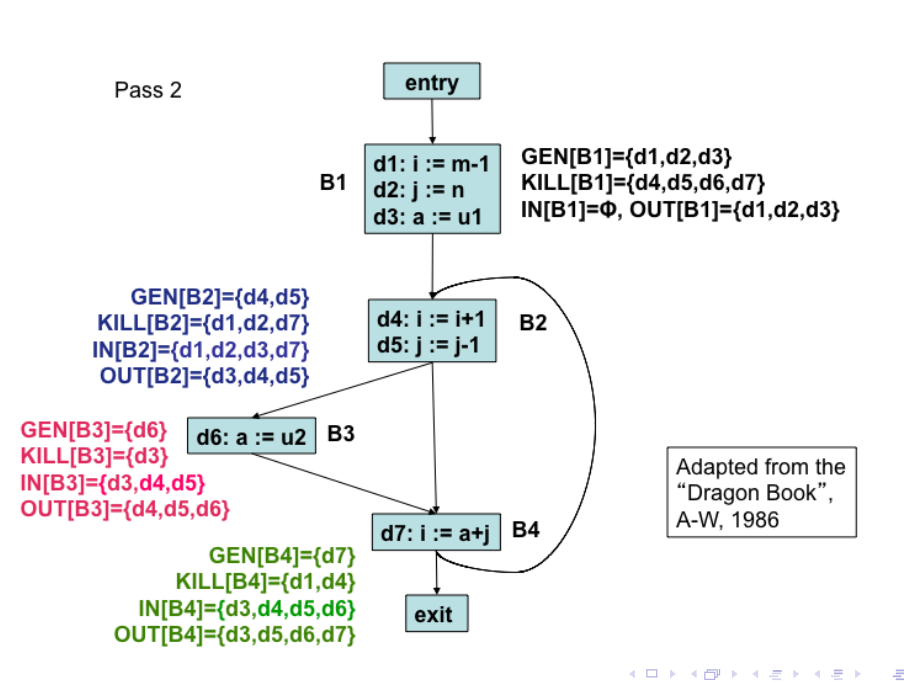
\includegraphics[width=0.4\textwidth]{Images/reaching2.png}
    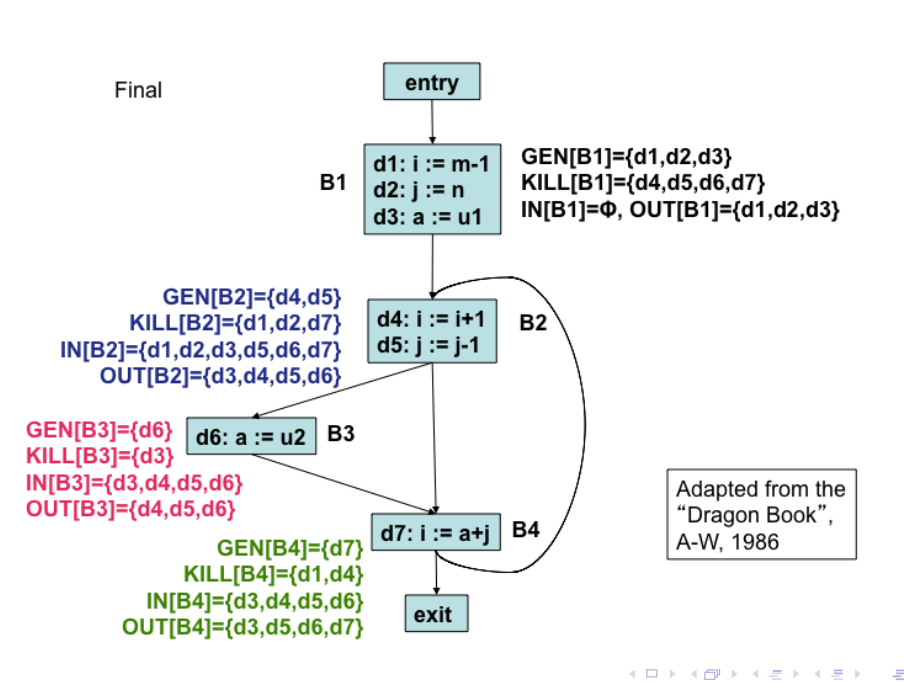
\includegraphics[width=0.4\textwidth]{Images/reaching3.png}
    \caption{Reaching Definitions}
    \label{fig:ReachingDefinitions}
\end{figure}

\newpage

In Pass 1, we initialize $IN(B) = \phi$ for all blocks and compute $OUT(B)$ using $GEN$, $KILL$ and $IN$ values. Now we repeat the process until $IN$ and $OUT$ values stabilize which in this case takes 3 iterations. \\

\subsection*{Iterative Algorithm for computing Reaching Definitions}
1. for each block $B$ initialize $IN(B) = \phi$ and $OUT(B) = GEN(B)$. \\
2. while there is a block $B$ such that $OUT(B)$ changes, do the following for each block $B$: \\
\begin{itemize}
    \item $IN(B) = \bigcup_{p \in pred(B)} OUT(p)$
    \item $OUT(B) = GEN(B) \cup (IN(B) - KILL(B))$
\end{itemize}

GEN, KILL, IN, OUT are all represented as bit vectors with one bit for each definition in the flow graph which is shown in following figure. \\

\begin{figure}[h]
    \centering
    \includegraphics[width=0.4\textwidth]{Images/bitVector.png}
    \caption{Bit Vector Representation}
    \label{fig:BitVector}
\end{figure}

\subsection*{Use-Definition Chains (u-d chains)}\
Convenient way to store reaching definitions once they are computed. A u-d chain is a \textbf{list of a use of a variable} and all the definitions that reach that use. \\

\begin{figure}[h]
    \centering
    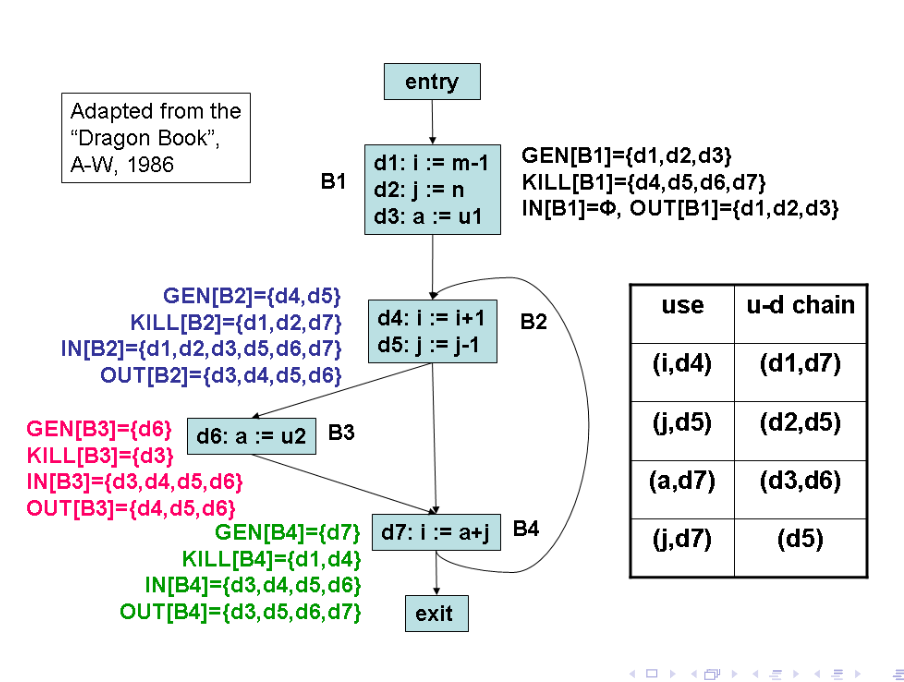
\includegraphics[width=0.4\textwidth]{Images/udchain.png}
    \caption{Use-Definition Chains}
    \label{fig:udChain}
\end{figure}

\subsection*{Construction of ud chains}
We need to consider 3 cases while constructing use-def chains which are as follows:

\begin{figure}[h]
    \centering
    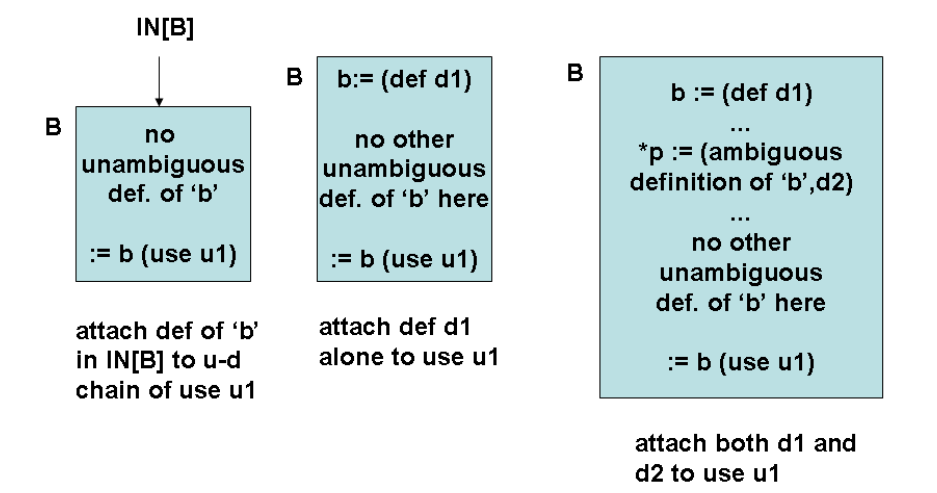
\includegraphics[width=0.6\textwidth]{Images/udchain2.png}
    \caption{Construction of ud chains}
    \label{fig:udChain}
\end{figure}

\section*{Available Expression Computation}
This computation is necessary to handle \textcolor{red}{common subexpression elimination} optimization. This is again a forward flow problem with $\cap$ as Confluence operator. \\
An Expression $E_x$ is said to be available at a point $p$ if every path (may contain cycle) from initial node which reaches $p$ evaluates $E_x$ somewhere along the path before reaching $p$. There can be multiple evaluations of $E_x$ but after last such evaluation there are no assignments to any of the variables in $E_x$. \\

\begin{figure}[h]
    \centering
    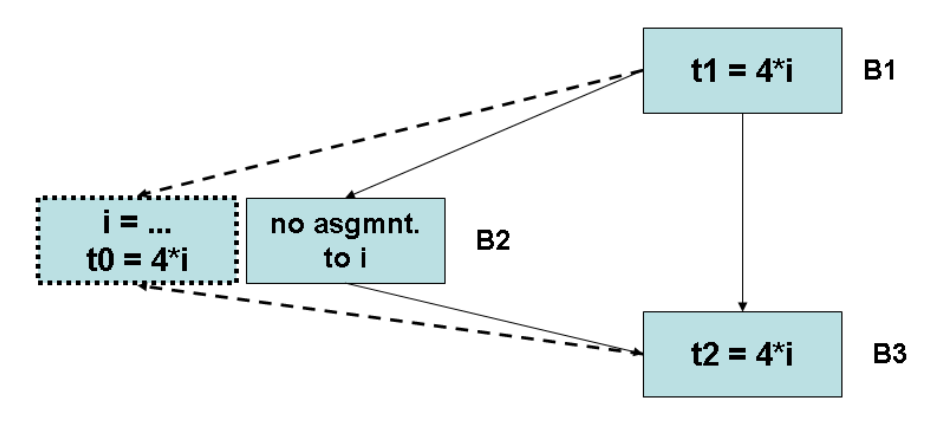
\includegraphics[width=0.3\textwidth]{Images/available1.png}
    \caption{Available Expressions}
    \label{fig:AvailableExpressions}
\end{figure}

In the figure above we can see that if we take path $B_2$ right then first evaluation to $4*i$ is in $B_1$ and it is available at $B_2$. If we take path $B_2$ left then first evaluation to $4*i$ then there is reassigment to $i$ and $4*i$ is again computed, hence it is available at $B_2$ in this case as well. In this case last evaluation of the expression is in $B_2$ and after the last evaluation there was no further re assignment to $i$.\\

A block kills $E_x$ if it assigns to any of the variables in $E_x$. For example consider $E(x,y) = x+y$. A block kills $E(x,y)$ if it assigns to $x$ or $y$. A block generates $E_x$ if it computes $E_x$ and does not kill it. \\

\subsection*{Data Flow Equations for Available Expressions}
The data flow equations are as follows: \\
1. $IN(B) = \bigcap_{p \in pred(B)} OUT(p)$ where $B$ is not the entry block. \\
2. $OUT(B) = \text{e\_gen} (B) \cup (IN(B) - \text{e\_kill}(B))$ \\
3. $IN(B_1) = \phi$ where $B_1$ is the entry block. \\
4. $IN(B) = U$, for $B \neq B_1$ \textcolor{red}{(Initialization)} \\

$IN(B_1)$ is always $\phi$, U is the set of all expressions 

\subsection*{Computing e\_gen and e\_kill}

\begin{figure}[h]
    \centering
    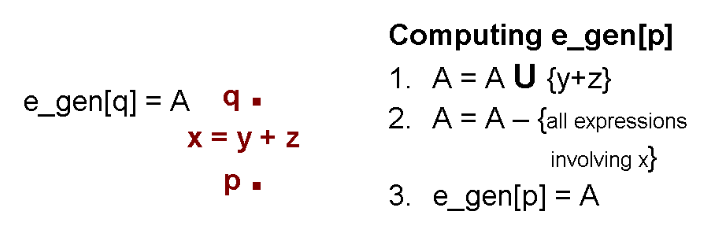
\includegraphics[width=0.4\textwidth]{Images/egen.png}
    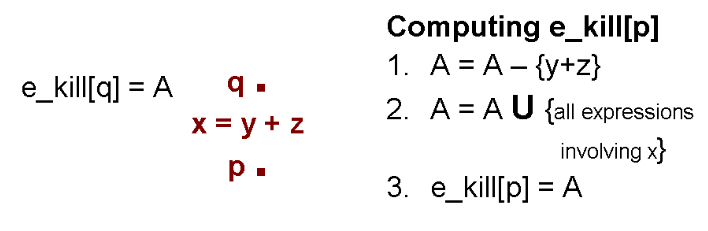
\includegraphics[width=0.4\textwidth]{Images/ekill.png}
    \caption{Computing e\_gen and e\_kill}
    \label{fig:AvailableExpressions}

\end{figure}

In the left figure we did $A = A - \{ \text{all expressions involving x} \}$ because of re assignment to $x$. In the right figure we did $A = A - \{y+z\}$ because in this case $A$ is set of killed expressions and $\{y+z\}$ is generated and due to re assignment to $x$, all expressions involving $x$ are added to $A$. Also for the statements of the form $x=a$, the step 1 of both algorithms shown does not apply. \\

\subsection*{Iterative Algorithm for Computing Available Expressions}
Algorithm 1: \\
1. for each block $B \neq B_1$ do $OUT(B) = U - e\_kill(B)$ \\
2. while there is a block $B$ such that $OUT(B)$ changes, do the following for each block $B$: \\

\begin{itemize}
    \item $IN(B) = \bigcap_{p \in pred(B)} OUT(p)$
    \item $OUT(B) = \text{e\_gen}(B) \cup (IN(B) - \text{e\_kill}(B))$
\end{itemize}

Algorithm2: \\
1. for each block $B \neq B_1$ do $IN(B) = U$ \\
2. while there is a block $B$ such that $OUT(B)$ changes, do the following for each block $B$: \\

\begin{itemize}
    \item $OUT(B) = \text{e\_gen}(B) \cup (IN(B) - \text{e\_kill}(B))$
    \item $IN(B) = \bigcap_{p \in pred(B)} OUT(p)$
\end{itemize}

In Algorithm 2, we have initialized $IN(B) = U$ first, and the only change in while loop is that $OUT(B)$ will be computed first and then $IN(B)$ will be computed. \\

\subsection*{Why not $IN(B) = \phi$ ?}
This initialization can be restrictive. We will get a valid solution, but it is possible that it may not be the largest possible solution. We require largest possible solution so that we can eliminate as many common subexpressions as possible. \\

\newpage
\begin{figure}[h]
    \centering
    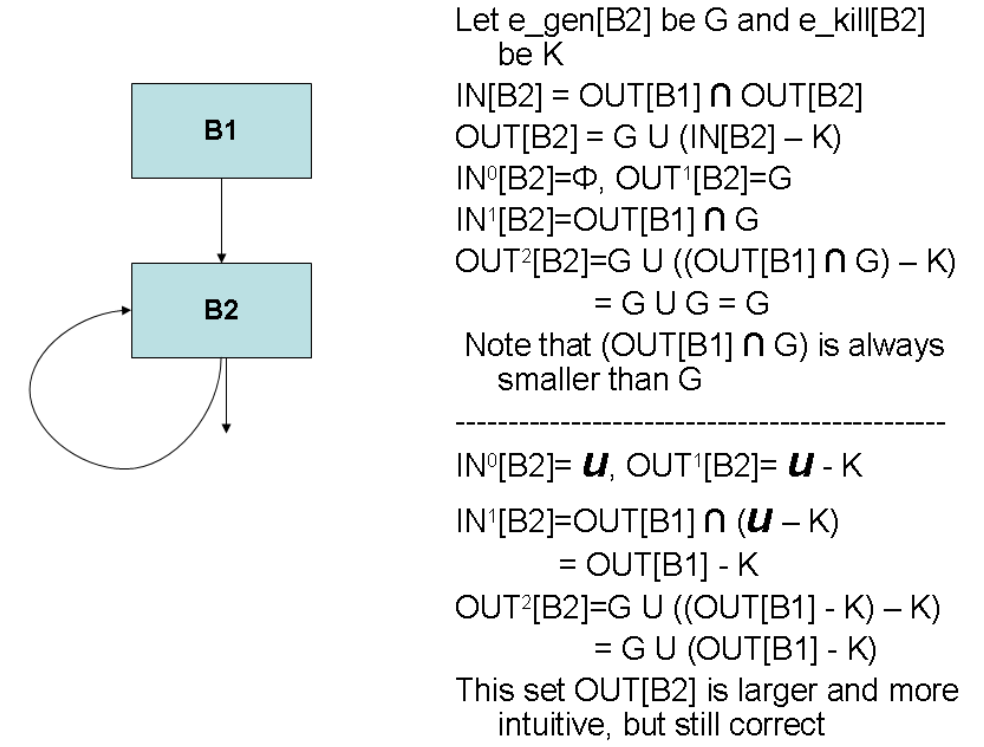
\includegraphics[width=0.7\textwidth]{Images/phi.png}
    \caption{Why not $IN(B) = \phi$ ?}
    \label{fig:AvailableExpressions}
\end{figure}

\begin{figure}[h]
    \centering
    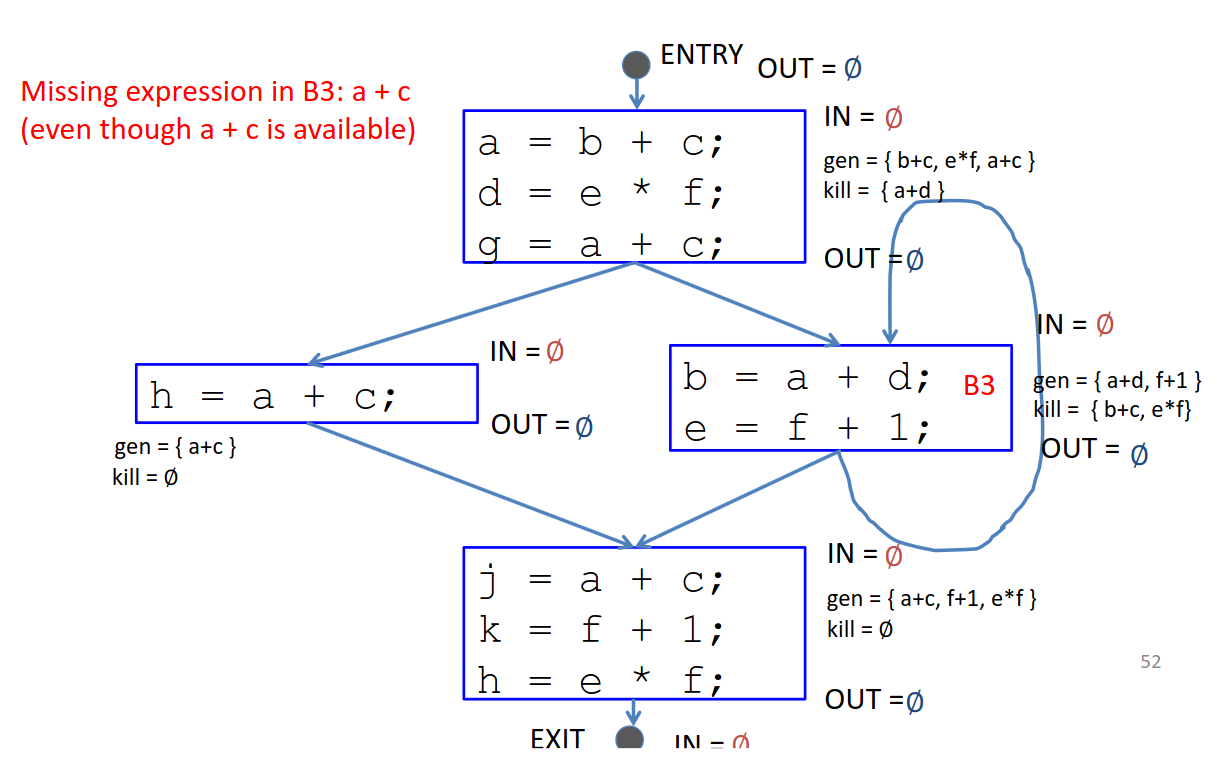
\includegraphics[width=0.7\textwidth]{Images/example.png}
    \caption{Available Expressions}
    \label{fig:AvailableExpressions}
\end{figure}

In above figure an example is given in which there is a available expression but it is not computed because of initialization with $\phi$. \\

\section*{Live Variable Analysis}
We say a variable $x$ is live at a point $p$, if the value of $x$ at $p$ could be used at some path in the flow graph starting at $p$, otherwise $x$ is dead at $p$. In this case the domain of the data flow values is sets of variables. This is backward data flow problem, with confluence operator as $\cup$. \\

\subsection*{Notations}
$IN(B)$ is the set of variables live at the beginning of block $B$ and $OUT(B)$ is the set of variables live at the end of block $B$. DEF(B) is the set of variables which are assigned in B prior to being used where as $USE(B)$ is the set of variables whose values may be used prior to definition of the variable. \\

\subsection*{Data flow equations}
Inittialize $IN(B) = \phi$ for all blocks $B$. Then we have: \\
1. $OUT(B) = \bigcup_{s \in succ(B)} IN(s)$ \\
2. $IN(B) = USE(B) \cup (OUT(B) - DEF(B))$ \\

\begin{figure}[h]
    \centering
    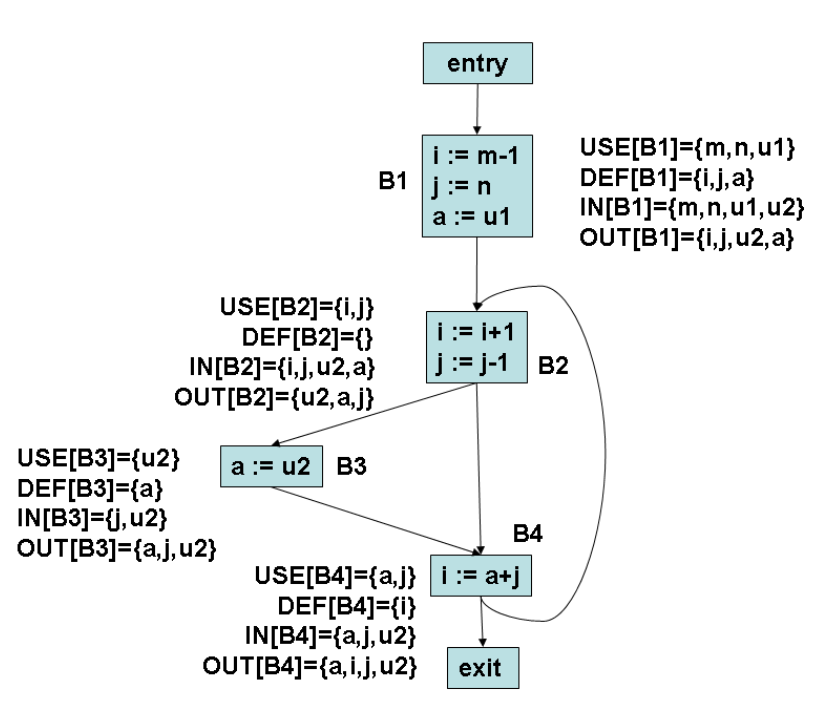
\includegraphics[width=0.3\textwidth]{Images/live.png}
    \caption{Final Live Variable Analysis after stabilization}
    \label{fig:LiveVariableAnalysis}
\end{figure}

Above figure shows the live variable analysis for a simple flow graph. Consider Block $B_2$, we can see that $i,j$ are used before assignment, hence they are in $USE(B_2)$. Similarly in $B_4$ - $a,j$ both are used before assignment and $i$ is assigned before use, hence $a,j \in USE(B_4)$ and $i \in DEF(B_4)$. \\

\subsection*{Definition Use Chains}
In this for each defintion we wish to attach the statement numbers of the uses of that defintion. This information is represented as sets of $(x,s)$ pairs where $x$ is the variable used in the statement $s$. In live variable analysis, we need information on whether a variable is used later but in $(x,s)$ computation we also need the statement number of the uses.

\subsection*{Data Flow Analysis for $(x,s)$ pairs}
Domain is $(x,s)$ pairs and this is again a backward data flow problem with confluence operator as $\cup$. \\ 

Here are some notations: \\
1. $USE(B)$ is the set of $(x,s)$ pairs $s$ is a statement in $B$ which uses $x$ before any reassignment to $x$ in $B$.\\ 
2. $DEF(B)$ is the set of $(x,s)$ pairs $s$ where is a statement number which uses $x$, $s$ is not in $B$ but $B$ contains a defintion of $x$ . \\ 
3. $IN(B)$ is the set of $(x,s)$ pairs such that statement $s$ uses $x$ and there is no re assignment to $x$ from beginning of $B$ to $s$. \\ 
4. $OUT(B)$ is the set of $(x,s)$ pairs such that statement $s$ uses $x$ and there is no re assignment to $x$ from ending of $B$ to $s$. \\

\begin{figure}[h]
    \centering
    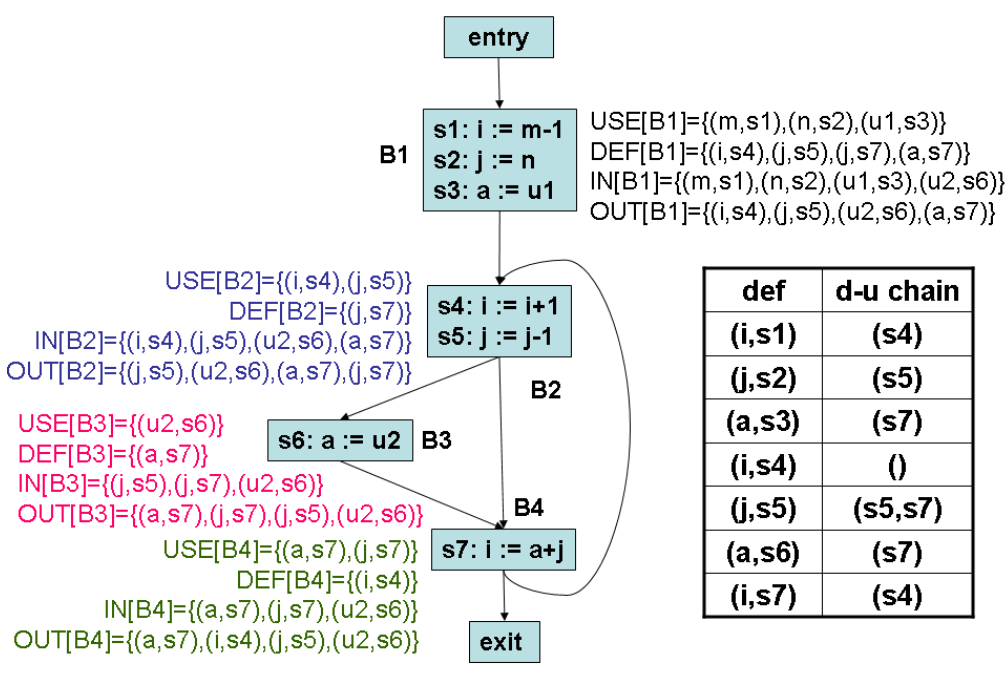
\includegraphics[width=0.3\textwidth]{Images/duchain.png}
    \caption{Definition Use Chains}
    \label{fig:DefUse}
\end{figure}

Data Flow equations remain same as live variable analysis but the domain is $(x,s)$ pairs. Once $IN(B)$ and $OUT(B)$ are computed for $(x,s)$ pairs, we can construct definition use chains. as follows: \\

\subsection*{Construction of Definition Use Chains}

\begin{figure}[h]
    \centering
    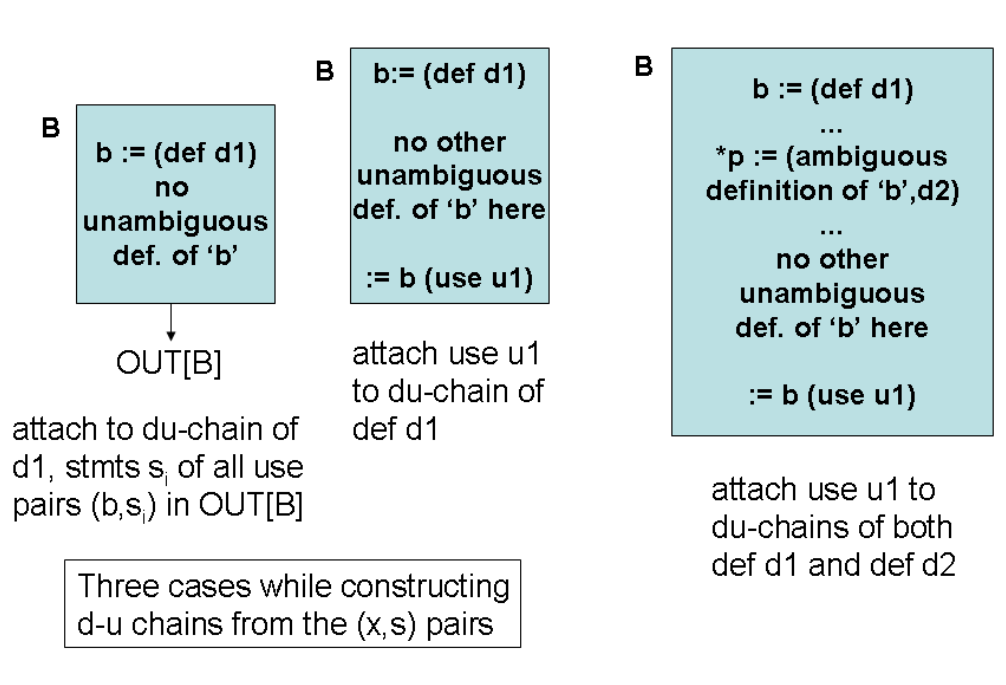
\includegraphics[width=0.5\textwidth]{Images/duchain2.png}
    \caption{Construction of Definition Use Chains}
    \label{fig:DefUse}
\end{figure}

\end{document}
